\documentclass[12pt,letterpaper]{article}
\usepackage{natbib}

%Packages
\usepackage{xcolor}
\usepackage{color,soul}
\usepackage{pdflscape}
\usepackage{fixltx2e}
\usepackage{textcomp}
\usepackage{fullpage}
\usepackage{float}
\usepackage{latexsym}
\usepackage{url}
\usepackage{epsfig}
\usepackage{graphicx}
\usepackage{amssymb}
\usepackage{amsmath}
\usepackage{bm}
\usepackage{array}
\usepackage[version=3]{mhchem}
\usepackage{ifthen}
\usepackage{caption}
\usepackage{hyperref}
\usepackage{amsthm}
\usepackage{amstext}
\usepackage{enumerate}
\usepackage[osf]{mathpazo}
\usepackage{dcolumn}
\usepackage{lineno}
\usepackage{dcolumn}
\usepackage{hyphenat}
\usepackage[T1]{fontenc}
\usepackage{textcomp}
\newcolumntype{d}[1]{D{.}{.}{#1}}

\pagenumbering{arabic}


%Pagination style and stuff
\linespread{2}
\raggedright
\setlength{\parindent}{0.5in}
\setcounter{secnumdepth}{0} 
\renewcommand{\section}[1]{%
\bigskip
\begin{center}
\begin{Large}
\normalfont\scshape #1
\medskip
\end{Large}
\end{center}}
\renewcommand{\subsection}[1]{%
\bigskip
\begin{center}
\begin{large}
\normalfont\itshape #1
\end{large}
\end{center}}
\renewcommand{\subsubsection}[1]{%
\vspace{2ex}
\noindent
\textit{#1.}---}
\renewcommand{\tableofcontents}{}
%\bibpunct{(}{)}{;}{a}{}{,}

%---------------------------------------------
%
%       START
%
%---------------------------------------------

\begin{document}

%Running head
\begin{flushright}
Version dated: \today
\end{flushright}
\bigskip
\noindent RH: disparate views on disparity.

\bigskip
\medskip
\begin{center}

\noindent{\Large \bf Disparate views on disparity.} 
\bigskip

\noindent {\normalsize \sc Thomas Guillerme$^1$$^,$$^*$, Natalie Cooper$^2$, ..., Philip Donoghue$^3$}\\
\noindent {\small \it 
$^1$Imperial College London, Silwood Park Campus, Department of Life Sciences, Buckhurst Road, Ascot SL5 7PY, United Kingdom.\\}
\end{center}
\medskip
\noindent{*\bf Corresponding author.} \textit{guillert@tcd.ie}\\  
\vspace{1in}

%Line numbering
\modulolinenumbers[1]
\linenumbers

%---------------------------------------------
%
%       ABSTRACT
%
%---------------------------------------------

\newpage
\begin{abstract}

\begin{enumerate}
    blablalbalba
\end{enumerate}

\end{abstract}

\noindent (Keywords: disparity)\\

\vspace{1.5in}

\newpage 

%---------------------------------------------
%
%       INTRODUCTION
%
%---------------------------------------------

\section{Introduction}
\label{text:intro}

Biodiversity is not a smooth gradient of forms, functions, ecologies, behaviours, etc., but it is rather variable and discontinuous. %TG: Actually is it?
This is at the base of biological sciences and is linked to the concept of disparity \citep{Wills2001,Hopkins2017} with the observation that some groups of species are more similar or dissimilar than others.
This diversity in morphologies is in fact proper in nature and decoupled from taxonomic diversity: some groups may exhibit low diversity of species by high diversity of shapes \citep[or the other way around]{ruta2013,hopkinsdecoupling2013}.
In palaeobiology, this concept, has been studied since the 90s describing \citep{gould1989wonderful,gould1991disparity,briggs1992morphological,Wills1994,Foote01071994,Foote29111996,jernvall1996molar,foote1997evolution} and as been extended with modifications to macroevolutionary analysis in general since the 2000s (whether based on continuous traits; e.g. \citealt{Harmon961,geiger2008}; or on geometric morphometrics; e.g. \citealt{claude2008morphometrics,zelditch2012geometric,adams2013geomorph,adams2017geometric}).

Since then, morphological disparity has been used for testing a vast array of biological hypotheses such as: how did body plans evolve through time? \citep{Wesley-Hunt2005}; why does some morphologies exist and not other? \cite{gerber2017geometry}; what is the tempo and mode of morphological innovations through time? \citep{Hughes20082013}; what is the effect of mass extinction on disparity? \citep{halliday2016eutherian}; how does competition between groups affect disparity? \citep{Brusatte12092008}; how did morpho-ecological niches get filled through time? \citep{price2014niche}; and many more.
%
This apparent versatility of morphological disparity analysis led to a phenomenal amount of papers based on disparity methods (Fig. \ref{Fig:GoogleOccurences})!
%
However, ``a lot of disparity studies are inductive fishing trips and are not often designed to test a specific hypothesis.''
%
Indeed, compared to the vast amount of publication using morphological disparity, only a handful highlight/solve problems and propose hypothesis testing.

\begin{figure}[!htbp]
\centering
   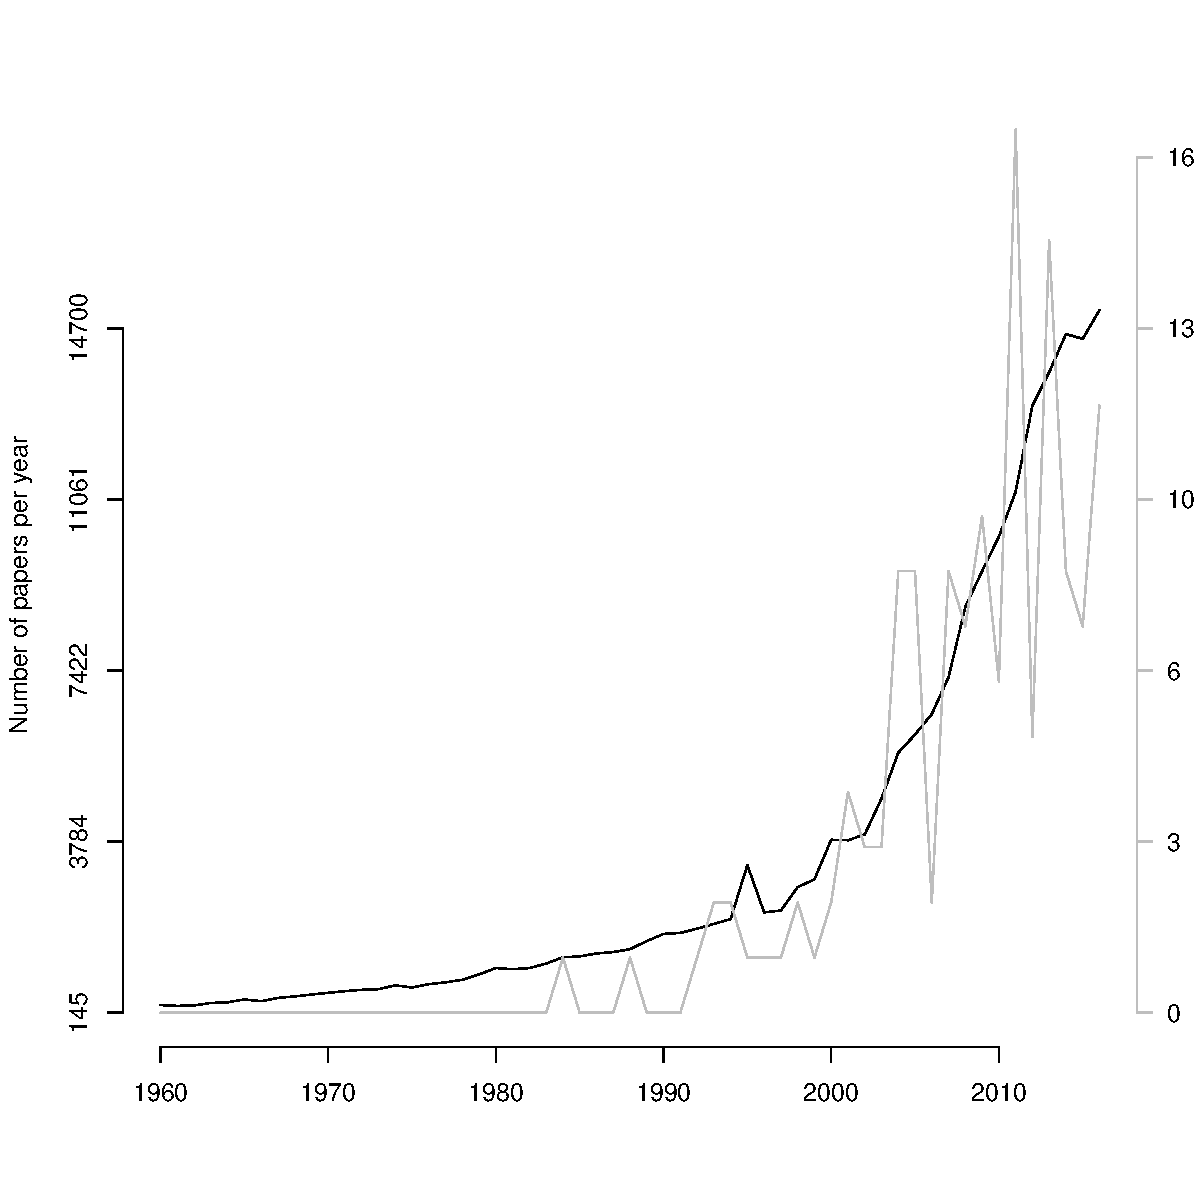
\includegraphics[width=1\textwidth]{Figures/GoogleScholarOccurences.pdf} 
\caption{Number of papers on Google Scholar matching the search ``morphological disparity'' per year. In black, the match is in the paper and in grey, in the title. We collected the number of matches per year from 1960 to 2016 in Google Scholar for the terms "morphological disparity" both in the text (fuzzy matching) or in the title (exact matching). The data was collected on the 1st of November 2017.}
\label{Fig:GoogleOccurences}
\end{figure}


\section{What actually \textit{is} disparity?}

\cite{prentice2011} define disparity as: ``a term widely (albeit not always consistently) used to describe the range of forms in a group of organisms, or the difference among different body plans''.
Disparity can describe either the metric (\citealt{Wills2001}; or index \citealt{Hopkins2017}) or the whole pipeline \citep{zelditch2012geometric,lloyd2016estimating}.
To assess the usage of disparity in different published studies, we collected methodological data from the 500 first Google Scholar results for the key words ``morphological disparity'' per order of appearance (accessed on the 1st of November 2017).
For the 230 relevant papers among the 500 matches, we collected the following methodological data: (1) What was the focal biological group? ; (2) What kind of data was measured (e.g. landmarks, discrete data, etc.)?  ; (3) Was data collected on the full organism or not? ; (4) How was the morphospace explicitly defined (e.g. PCA, PCO, MDS, etc.)? ; (5) How was the disparity metric(s) explicitly defined? ; (6) Which statistical test was applied to test the disparity related hypothesis? ; (7) Was phylogeny taken into account or not?
We used only the explicit definition of the morphospace and the disparity metric(s) in this search since a few number of papers had a vague definition of either or both (e.g. a disparity metric was measured but not described anywhere in the paper).
The remaining 270 matches were disparity was mentioned but not measured felt in the following categories: papers out of topic, papers mentioning morphological disparity without measuring it, review papers, papers not accessible (either through a broken link or a paywall) or referenced citation without the paper (as a Google Scholar match).
To reduce the amount of categories for the 230 recorded methods, we concatenated different methods in a smaller number of categories (see supplementary materials and \url{https://github.com/TGuillerme/Disparity_Working_Group/blob/master/Analysis/data_cleaning.Rmd}).

\begin{figure}[!htbp]
\centering
   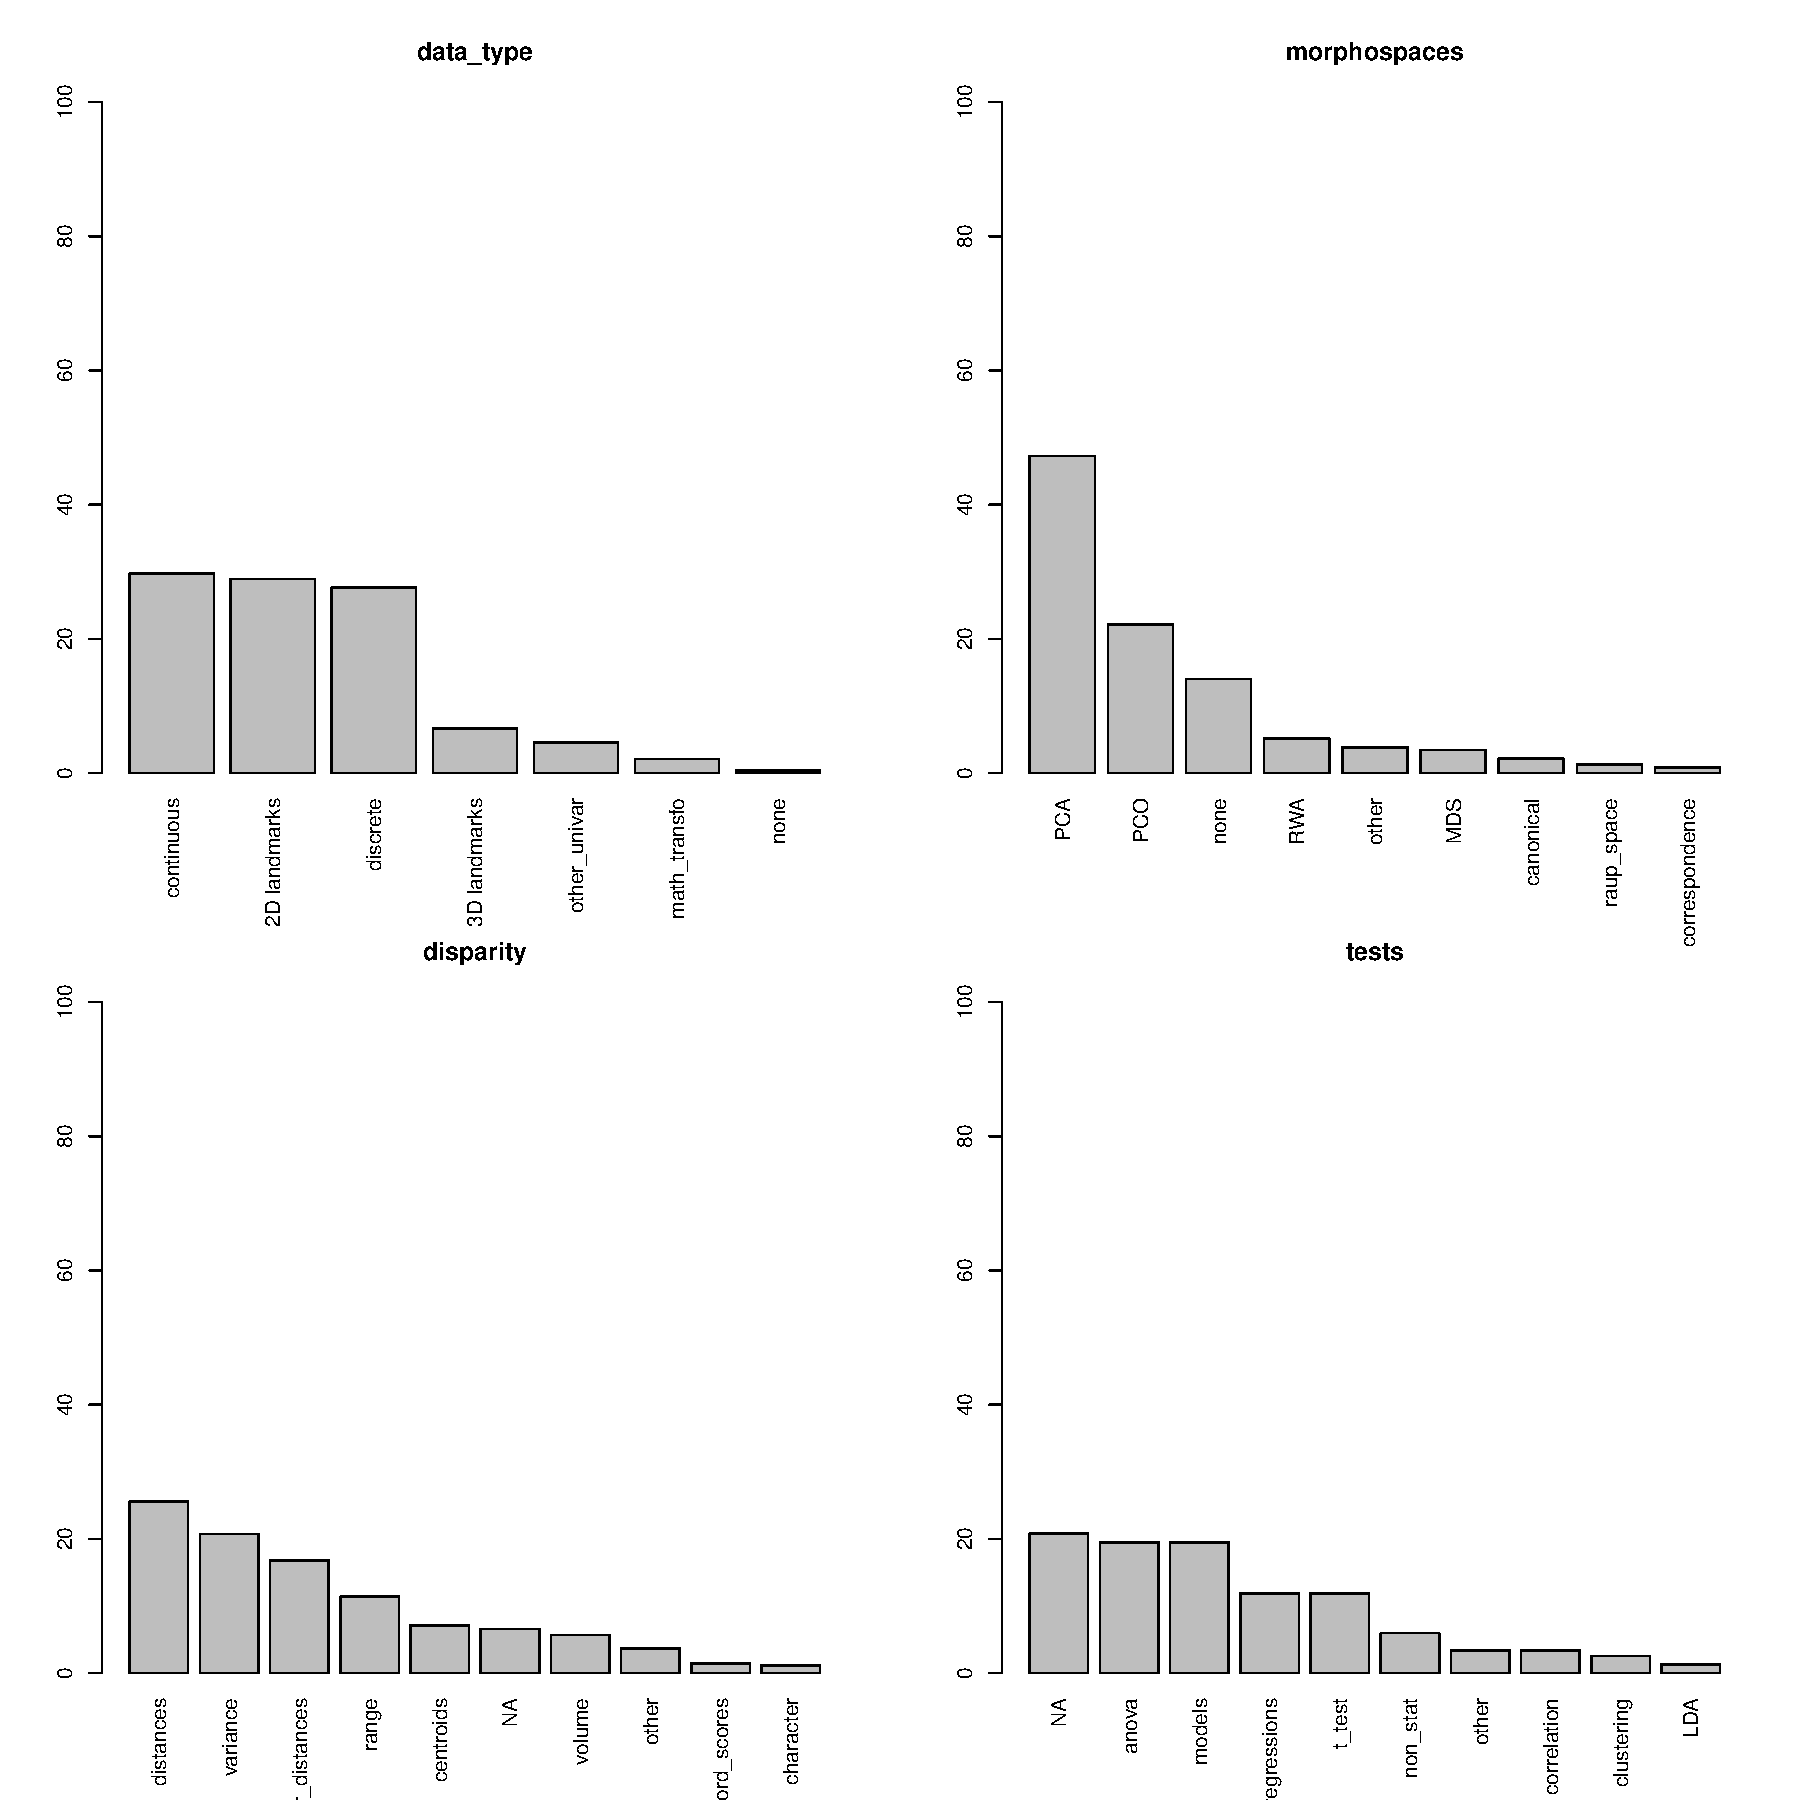
\includegraphics[width=1\textwidth]{Figures/MethodsProportions.pdf} 
\caption{Disparity methods proportional usage: (1) Data type: which input data was used (...); (2) Morphospace: how was the morphospace obtained (...); (3) disparity: what type of disparity metric was calculated (...); (4) test: what type of test was applied (...).}
\label{Fig:MethodsProportions}
\end{figure}

From the collected data, we can highlight the use of three main different disparity analysis with their associated data/morphospace/metric/tests and related to specific methodological implementations.

\begin{itemize}
    \item \textbf{The ``\texttt{Claddis}'' approach:} this group of methods uses discrete morphological data (sometimes referred to as ``Cladistic'' characters) for the full organisms to build a PCO from the organism's pairwise distance as a morphospace. Disparity is then often measured as a variation of the ordinated matrix dimensions' variances or ranges (e.g. the sum of variance or/and the sum of ranges). Hypothesis are often tested using multivariate ANOVAs on the pairwise distance matrix or by simply comparing the confidence intervals overlap of the disparity from different groups. 

    \item \textbf{The ``\texttt{geomorph}'' approach:} this group of method is based on landmark data (2D or 3D) on parts of the organism studied usually the skull) and use a Procrustes transformation of the landmarks that are then directly ordinated using a PCA (but sometimes RWA). Disparity is often measured as a distance metric (e.g. the distance between the species and a point in the morphospace such as its centroid). Hypothesis are then tested using ANOVA type tests with usually no phylogenetic correction (although phylogeny is sometimes used to correct the morphospace).

    \item \textbf{The ``\texttt{approach}'' approach:} this method can directly use continuous or discrete data for the full organism without any ordination (but not necessarily), and will measure disparity as the average pairwise distance between species (whether euclidean or any other type of distance). Hypothesis of higher/lower disparity can then be measured using null evolutionary models.
\end{itemize}

%
The advent of these three approaches coincides with the explosion of disparity analysis (Fig. \ref{Fig:GoogleOccurences}) and suggest a high popularity of disparity analysis.
%
Unfortunately, however, few actual tests have been performed on whether any of these approaches \textit{actually} allows to tackle the classic disparity questions (see \ref{text:intro}{Introduction}).
Are all these methods the right tools to answer these questions are they mere ``inductive fishing trips'' used to describe the data rather than testing any of the hypothesis related to the disparity questions?

\section{Does data used in disparity analysis allows to test hypothesis?}
In fact, the question of which data to analyse \citep{hetherington2015cladistic} and which part of the data to use has been analysed \citep{hopkins2017well} has rarely been assessed.
Can the data used in disparity studies actually test the phenomenon researchers are trying to capture?

For example, when studying discrete morphological characters (often following the ``\texttt{Claddis}'' approach), the data used is often recycled data used for phylogenetic analysis.
These datasets are usually design to recover evolutionary history and differentiate clades and, often due to the preservations of the fossil record, are mainly based on hard tissue characters.
In phylogenetics, this artefact have been shown to be leading to measurable topological recovery error (for soft \textit{vs} hard characters; \citealt{sansomfossilization2013}; or dental \textit{vs} cranial characters \citealt{sansom2017dental}).
Therefore, is the morphospace composed of ``fossilisable'' characters enough for answering evolutionary hypothesis?
For example, are niche replacement hypothesis equivalent to fossilisable-character-based-niches replacement hypothesis?

Similarly, many studies in geometric morphometric are based solely on skull shape using landmark techniques combined with Procrustes superimposition \citep[the ``\texttt{geomorph}'' approach;][]{zelditch2012geometric,adams2017geometric}.
However, it has been shown that the whole skeleton displays different integrated modules with different specific evolutionary constraints leading to variable rates and modes of evolution (\citealt{Goswami20130254}; and this even at the cranial level \citealt{goswami2010influence}).
Is skull variation enough for measuring body plans variation through time for example?

In the case where disparity is measured a single continuous trait (or a collection of traits; following the ``\texttt{geiger}'' approach), for example in \cite{price2014niche}, beak and limb length as well as body mass are used to differentiate groups of birds and different zones in the morphospace can then be interpreted as different niches.
Is this set of traits studied in isolation sufficient to test niche occupancy hypothesis?

Additionally, in many cases, the disparity metrics and hypothesis are often based on a transformation of the data (pairwise distances, PCA, PCO, MDS, RWA, etc.).
Can these transformation readily reflect the raw data in our hypothesis?
For examples a morphospace as a pairwise matrix reflects the dissimilarity between the data, a morphospace based on an ordination reflects the variability within the data, a morphospace based on both reflects the variability within the dissimilarity, are each method reflecting that?

\section{Do the disparity metrics (or indices) really reflect variation in the studied phenomenon?}
From the 230 papers analysed, we found 104 unique combination's of metrics to measure disparity (Fig. \ref{Fig:MethodsProportions}).
Commonly, these metrics are used to approximate the volume occupancy within the morphospace \citep{Wills2001,DonohueDim,diaz2016global}.

However, it has been shown that different metrics reacts differently depending on the dataset \citep[][; and an anecdotal example in Fig. \ref{Fig:DimensionsEffect}]{Wills2001,Ciampaglio2001}.
For example metrics involving a product of aspects of the matrix (e.g. the volume, the product of the dimensions) are likely to suffer from the \textit{Curse of dimensionality} \citep{bellman1957dynamic} and will quickly tend to null values.
Some other metrics are not representing all the data captured in the morphospace (e.g. the sum or product of variance ignores the co-variance between dimensions).
Are these metrics as a description of the ordination a good proxy for the observed biological phenomenon?


\begin{figure}[!htbp]
\centering
   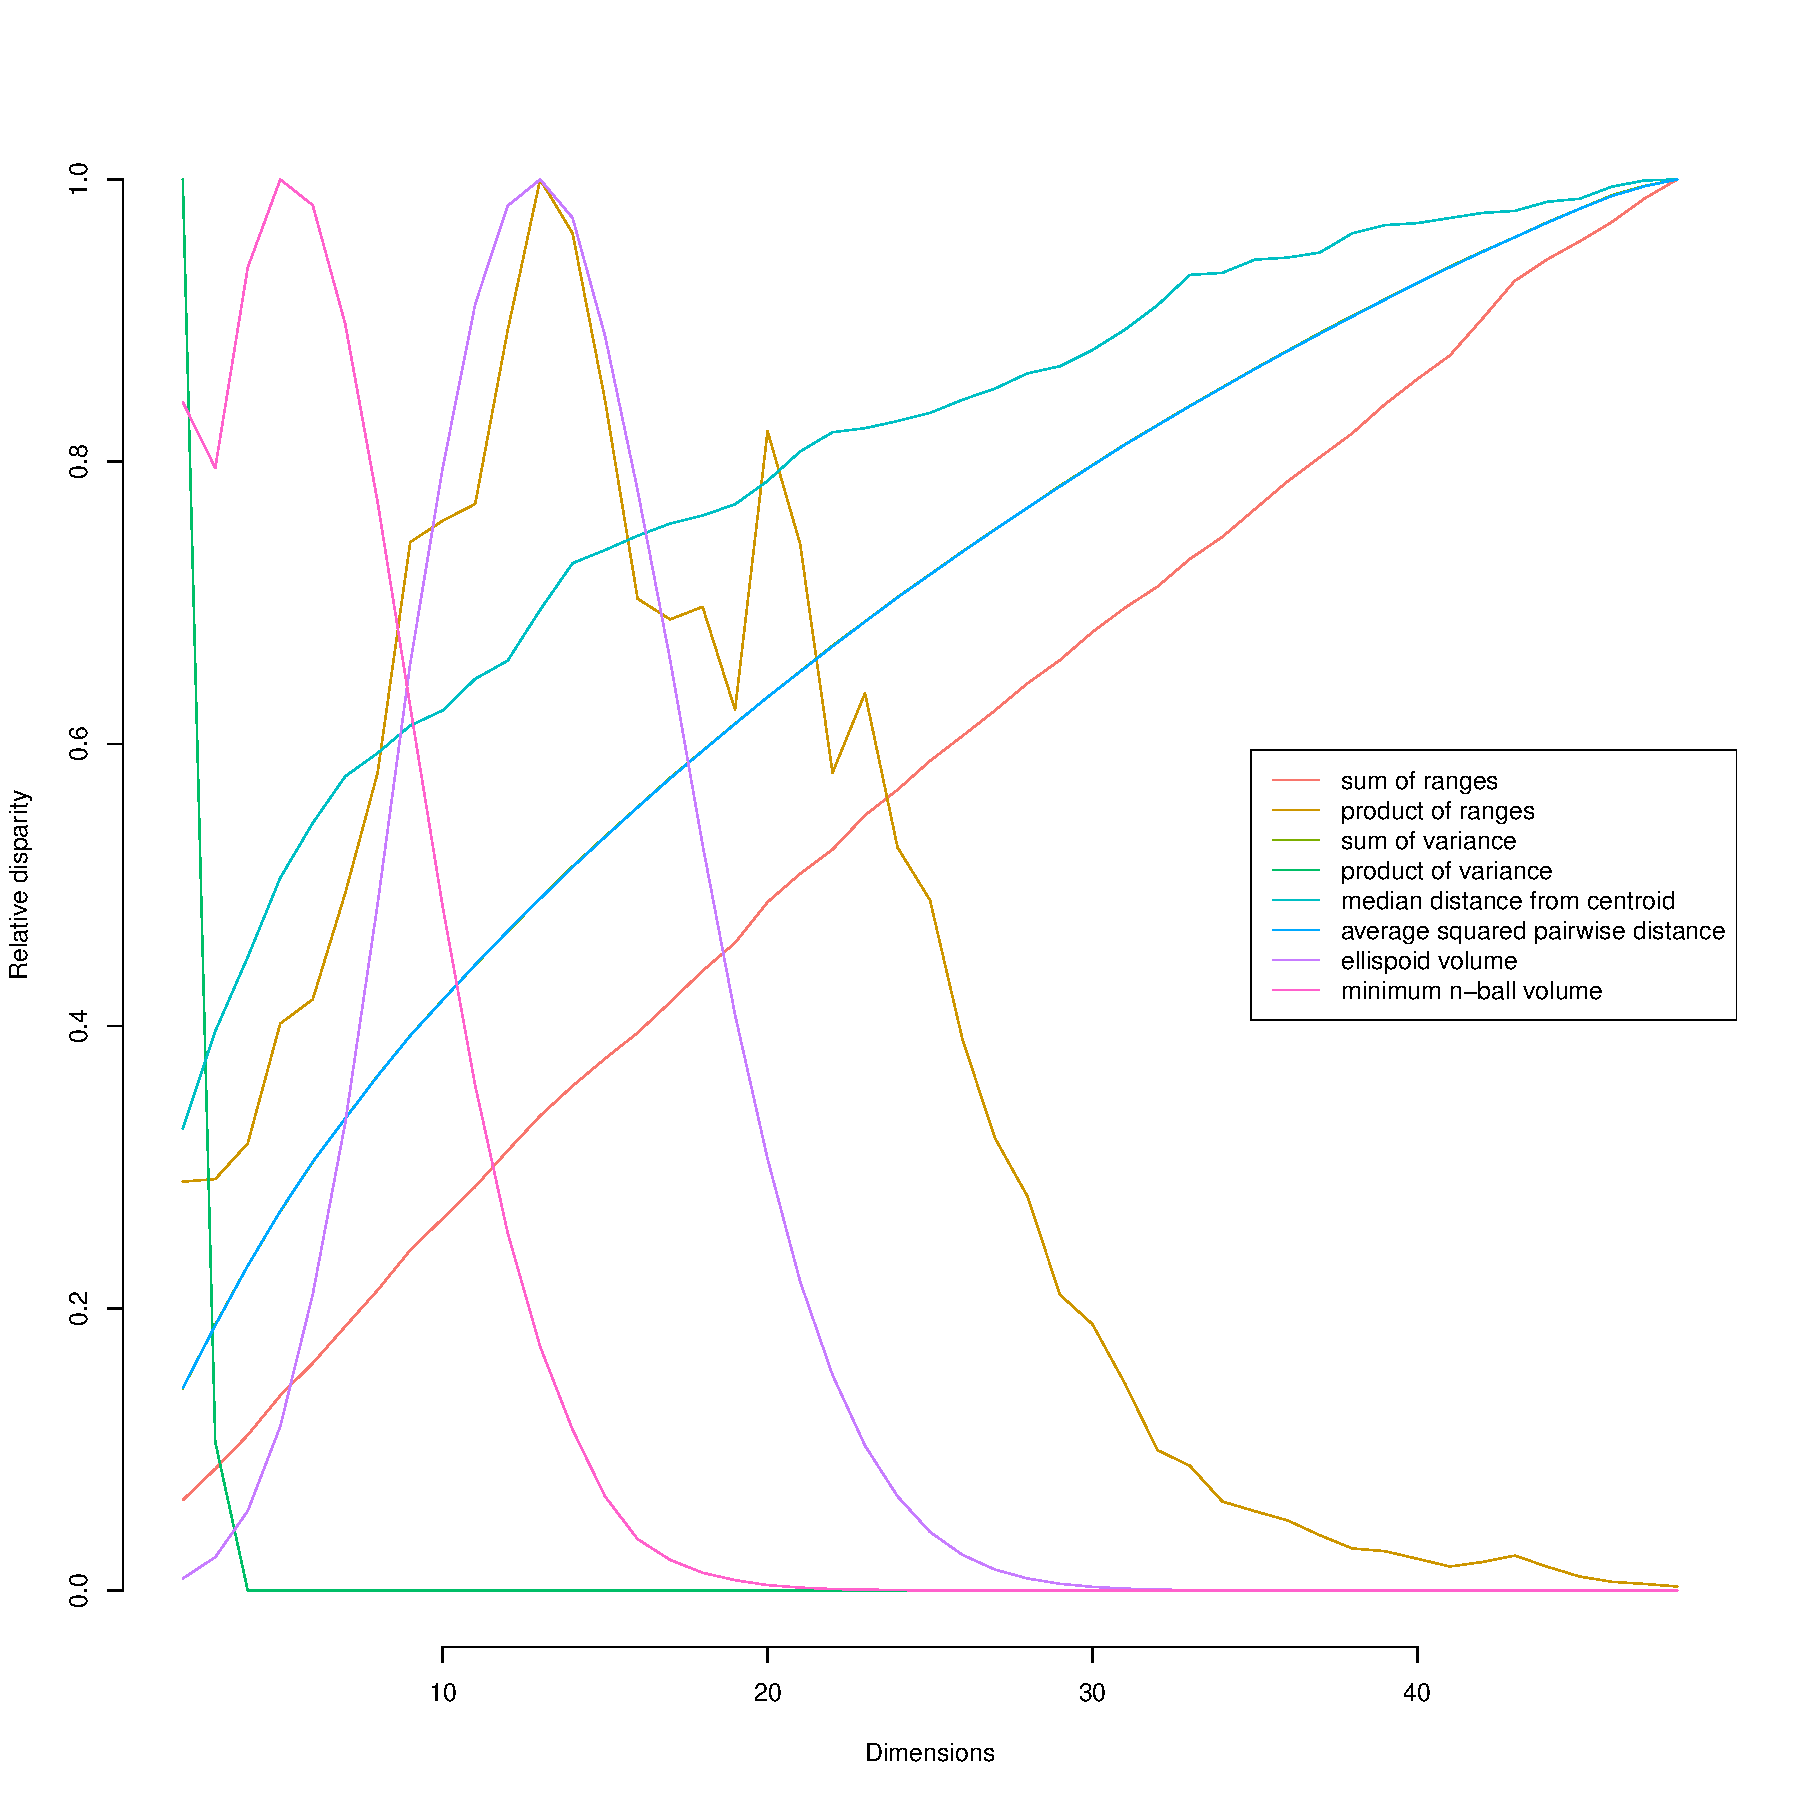
\includegraphics[width=1\textwidth]{Figures/DimensionsEffect.pdf} 
\caption{Effect of the number of dimensions on different disparity metrics (note that the sum of variance is equal to the average squared pairwise distance in this case).
The data used is one of the example datasets from the \texttt{dispRity R} package \citep[\texttt{BeckLee\_mat50};][]{beckancient2014,dispRityv02} composed of 50 elements and 48 dimensions obtained from a ordination (MDS) of the distance matrix of a discrete morphological character matrix.}
\label{Fig:DimensionsEffect}
\end{figure}

Despite these caveats, it is important to actually know what the metrics are measuring.
There has been some attempts to test that through simulations \citep{Ciampaglio2001,  gerber2017geometry} but it is still unclear which metric reflects the best the hypothesis test.
For example, the average squared pairwise distance (or the sum of ranges) are really popular \citep[e.g.][]{geiger2008} yet has been shown to be fairly senstive, at least in empirical data to the number of sampled taxa, the number of characters and the data completeness \citep[][; although effects were lesser in simulations]{Ciampaglio2001}.
More fundamentally, the question arises whether one disparity metric could be sufficient to describe changes in disparity?
Changes in multidimensions might not be readily grasped by unidimensional metrics!
For example, a given taxonomic group might have the exact same volume as another one yet be in a complete different part of the morphospace \citep[or even overlap or not depending on the dimensions;][]{davis2012acanthodes,brusatte50}.
In this case, it might more interesting to have multiple metrics (e.g. the position and the volume) [FABRE et. al in prep.] or to use distributions of metrics (e.g. what does the average distance between species or from a point really convey? Is the distribution not more interesting?).

Maybe we need metrics that fit explicitly our hypothesis (or fit our hypothesis directly to the metric).
For example, for competitive replacement, should we not measure whether group A occupies the same place as group B through time and whether that is due to competition or simply because any other place in the space cannot be occupied (and why are such spaces unoccupied)?


\section{Is the current statistical toolkit sufficient for testing disparity hypothesis?}
Are the methods used to test hypothesis in disparity actually testing what we think they’re testing (problem of multidimensional hypothesis)
What does an anova or related variance based test real infirm/confirms regarding the disparity questions?
How do we deal with bootstrapped data and pseudo-replications?
Can we realistically use univariate Gaussian models to test hypothesis based on multivariate, probably non-Gaussian data? \citep{blomberg2017beyond}

Should be take phylogeny into account? \citep{polly2013phylogenetic}



\section{What are we missing?}

\subsection{Learning lessons from other fields}
In ecology, disparity bears strong parallels with $\beta$-diversity in ecology (a measure of ecological communities (dis)similarity): one biological observation described by a vast array of metrics \citep{baselga2010partitioning, anderson2011navigating, donohue2016navigating}.

\section{Conclusion}
We need a more hypothesis driven way of analysing disparity.
Disparity methods should be the tool for answering disparity hypothesis, not merely a description of the data.




% \hl{[ADD Biological group, full organism and phylogeny in the supplementary]}

% \noindent \hl{\textit{These points should be developed during the meeting}}


% \subsection{Disparity data}
% The data used for disparity methods comes from three main sources:
% \begin{itemize}
%     \item Continuous data such as limb or body measurements \citep{slaterCetacean}.
%     \item Discrete morphological characters \citep[sometimes referred to as ``Cladistic'' characters; ][]{Brusatte12092008}.
%     \item Geometric morphometric data which is generally the Procrustes transformation of 2D or 3D landmarks \citep{cooney2017mega}.
% \end{itemize}

% However, data was by far not limited to these three categories (e.g. colours \citealt{maia2013key}; metabolic rate \citealt{nespolo2016studying} or chemicals signal \citealt{garcia2017heterogeneous}).

% \subsection{Morphospaces}
% \begin{itemize}
%     \item PCAs [CITE].
%     \item PCOs [CITE]
%     \item Pairwise distance matrices \citep[no ordination; ][]{Harmon961}.
% \end{itemize}

% But also RWA [CITE] or Raup-spaces [CITE].

% \subsection{Disparity metrics}
% Throughout the 230 analysed papers, we found 103 unique combinations of metrics!

% \begin{itemize}
%     \item Distances measurements between species or from a certain point in the morphospace [CITE].
%     \item Ranges and variances of each axis of the morphospace \cite{Wills2001,Ciampaglio2001}
%     \item Distance between species based on the pairwise distance matrix (not the ordinations) [CITE].
% \end{itemize}

% But also metrics based on the volume [CITE], the characters dissimilarity [CITE] or the coordinates of some axis of the ordination [CITE]

% \subsection{Disparity hypothesis}
% Describing the many outputs (what and how is it tested):

% \begin{itemize}
%     \item Variance based (ANOVA, etc.) [CITE].
%     \item Correlation based [CITE].
%     \item Regression based (PGLS, etc.) [CITE].
% \end{itemize}

% But also discriminant analysis [CITE] and clustering [CITE].

% Of course some studies use a combination of these three methods or none of them at all!

% Also, among each category XX\% of studies use multiple approaches.

% [ADD Biological group, full organism and phylogeny in the supplementary]

% \section{Expanding disparity}

% How to compare disparity between groups? Is disparity relative?

% How to compare disparity between methods?

% Can we really say things about competition when looking at disparity in a single group?

% Are all characters equal? Character contingency suggests otherwise

% What is the relationship between disparity and tree shape?

% Do we have a null model for investigating disparity?

% Can we really say things about competition when looking at disparity in a single group?


% \noindent \hl{\textit{Disparity in other fields}}

% In ecology, disparity bears strong parallels with $\beta$-diversity in ecology (a measure of ecological communities (dis)similarity): one biological observation described by a vast array of metrics \citep{baselga2010partitioning, anderson2011navigating, donohue2016navigating}.

% \section{Conclusion}

% A quick guideline for good disparity analysis:

% Maybe we need something like in Parham et al 2012 (Best Practices for Justifying Fossil Calibrations): an easy an identifiable description of the pipeline containing: 1) the type of data, 2) the morphospace and 3) the metric? 

\section{Acknowledgments}
The Royal Society.
TG acknowledge support from European Research Council under the European Union's Seventh Framework Programme (FP/2007 – 2013)/ERC Grant Agreement number 311092 awarded to Martin D. Brazeau.


\bibliographystyle{sysbio}
\bibliography{References}

\end{document}

